\section{Caligrafía}
\subsection{Caligrafía en dibujo técnico}
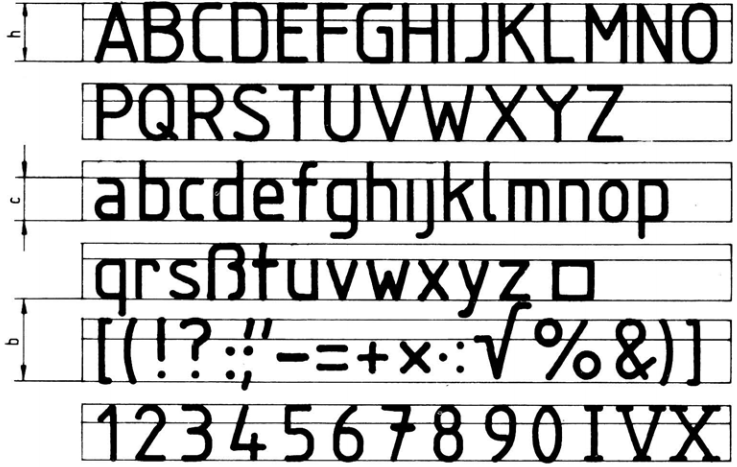
\includegraphics[width=0.9\textwidth]{images/05/caligrafia.png}


La letra técnica es parte integral de un dibujo, la utilidad de la letra técnica es indicar por escrito toda la información necesaria de un Dibujo y el nombre es porque el tipo de letras y números deben trazarse de acuerdo con las técnicas.
\begin{enumerate}
\item  Conocer sus formas y proporciones correcta.
\item Orden y sentido de los trazos.
\item Uniformidad (altura, inclinación, intensidad y peso de las líneas, espaciamiento entre letras y palabras, apariencia.)
\item La práctica persistente.
\end{enumerate}

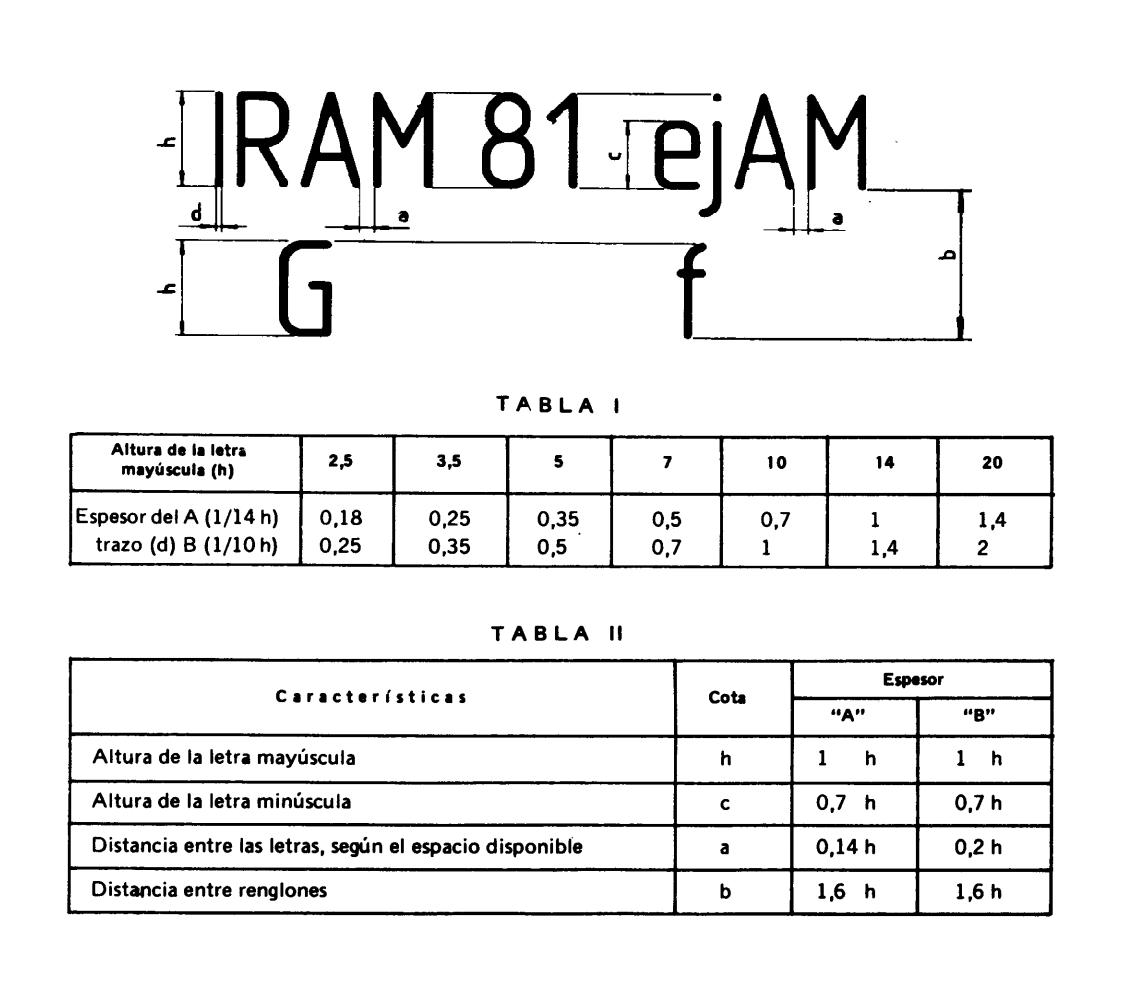
\includegraphics[width=0.9\textwidth]{images/05/dimensiones.png}

\subsection{
Ejercitación: }Completar los siguientes ejercicios de caligrafía, repitiendo el formato de letra. ( copiar lo mejor posible)

\newpage
\begin{tikzpicture}[remember picture, overlay, shift={(-3.6,-27.8)}]
\tikzstyle{every node}=[font=\Huge]
\draw [step=0.1,gray,line width=0.1mm] (2.5,4.5) grid (20,28.7) ;
\draw [step=1cm,black,line width=0.1mm] (2.5,4.5) grid (20,28.7) ;

\node at (5,28.3) [fontscale=4]{A A A A A A A};
\node at (3,27.3) [fontscale=4]{B};
\node at (3,26.3) [fontscale=4]{C};
\node at (3,25.3) [fontscale=4]{D};
\node at (3,24.3) [fontscale=4]{E};
\node at (3,23.3) [fontscale=4]{F};
\node at (3,22.3) [fontscale=4]{G};
\node at (3,21.3) [fontscale=4]{H};
\node at (3,20.3) [fontscale=4]{I};
\node at (3,19.3) [fontscale=4]{J};
\node at (3,18.3) [fontscale=4]{K};
\node at (3,17.3) [fontscale=4]{L};
\node at (3,16.3) [fontscale=4]{M};
\node at (3,15.3) [fontscale=4]{N};
\node at (3,14.3) [fontscale=4]{O};
\node at (3,13.3) [fontscale=4]{P};
\node at (3,12.3) [fontscale=4]{Q};
\node at (3,11.3) [fontscale=4]{R};
\node at (3,10.3) [fontscale=4]{S};
\node at (3,9.3) [fontscale=4]{T};
\node at (3,8.3) [fontscale=4]{U};
\node at (3,7.3) [fontscale=4]{V};
\node at (3,6.3) [fontscale=4]{W};
\node at (3,5.3) [fontscale=4]{X};
\end{tikzpicture}

\newpage
\begin{tikzpicture}[remember picture, overlay, shift={(-3.6,-27.8)}]
\tikzstyle{every node}=[font=\Huge]
\draw [step=0.1,gray,line width=0.1mm] (2.5,4.5) grid (20,28.7) ;
\draw [step=1cm,black,line width=0.1mm] (2.5,4.5) grid (20,28.7) ;

\node at (3,28.3) [fontscale=4]{Y};
\node at (3,27.3) [fontscale=4]{Z};
\node at (3,26.2) [fontscale=4]{a};
\node at (3,25.3) [fontscale=4]{b};
\node at (3,24.2) [fontscale=4]{c};
\node at (3,23.3) [fontscale=4]{d};
\node at (3,22.2) [fontscale=4]{e};
\node at (3,21.3) [fontscale=4]{f};
\node at (3,20.3) [fontscale=4]{G};
\node at (3,19.3) [fontscale=4]{h};
\node at (3,18.3) [fontscale=4]{i};
\node at (3,17.3) [fontscale=4]{j};
\node at (3,16.3) [fontscale=4]{k};
\node at (3,15.3) [fontscale=4]{l};
\node at (3,14.2) [fontscale=4]{m};
\node at (3,13.2) [fontscale=4]{n};
\node at (3,12.2) [fontscale=4]{o};
\node at (3,11.1) [fontscale=4]{p};
\node at (3,10.1) [fontscale=4]{q};
\node at (3,9.2) [fontscale=4]{r};
\node at (3,8.2) [fontscale=4]{s};
\node at (3,7.3) [fontscale=4]{t};
\node at (3,6.2) [fontscale=4]{u};
\node at (3,5.3) [fontscale=4]{v};
\end{tikzpicture}

\newpage
\begin{tikzpicture}[remember picture, overlay, shift={(-3.6,-27.8)}]
\tikzstyle{every node}=[font=\Huge]
\draw [step=0.1,gray,line width=0.1mm] (2.5,4.5) grid (20,28.7) ;
\draw [step=1cm,black,line width=0.1mm] (2.5,4.5) grid (20,28.7) ;

\node at (3,28.2) [fontscale=4]{w};
\node at (3,27.2) [fontscale=4]{x};
\node at (3,26.3) [fontscale=4]{y};
\node at (3,25.2) [fontscale=4]{z};
\node at (3,24.3) [fontscale=4]{1};
\node at (3,23.4) [fontscale=4]{2};
\node at (3,22.4) [fontscale=4]{3};
\node at (3,21.3) [fontscale=4]{4};
\node at (3,20.3) [fontscale=4]{5};
\node at (3,19.3) [fontscale=4]{6};
\node at (3,18.3) [fontscale=4]{7};
\node at (3,17.3) [fontscale=4]{8};
\node at (3,16.3) [fontscale=4]{9};
\node at (3,15.3) [fontscale=4]{\%};
\node at (3,14.3) [fontscale=4]{0};
\node at (4.2,13.3) [fontscale=4]{Escuela};
\node at (3.9,12.3) [fontscale=4]{4-239};
\node at (3.9,11.3) [fontscale=4]{Cerro};
\node at (3.2,10.3) [fontscale=4]{El};
\node at (4.8,9.3) [fontscale=4]{Sosneado};
\node at (4.1,8.2) [fontscale=4]{Dibujo};
\node at (4.3,7.3) [fontscale=4]{Técnico};
\node at (5,6.3) [fontscale=4]{pecuario};
\node at (4.7,5.2) [fontscale=4]{Caligrafía};
\end{tikzpicture}

